\let\negmedspace\undefined
\let\negthickspace\undefined
\documentclass[journal,12pt,onecolumn]{IEEEtran}
\usepackage{cite}
\usepackage{amsmath,amssymb,amsfonts,amsthm}
\usepackage{algorithmic}
\usepackage{tasks}
\settasks{label=\brak{\Alph*}, label-width=3ex, item-indent=0pt, column-sep=2em}
\usepackage{graphicx}
\graphicspath{{./figs/}}
\usepackage{textcomp}
\usepackage{xcolor}
\usepackage{txfonts}
\usepackage{listings}
\usepackage{enumitem}
\usepackage{mathtools}
\usepackage{gensymb}
\usepackage{comment}
\usepackage{caption}
\usepackage[breaklinks=true]{hyperref}
\usepackage{tkz-euclide} 
\usepackage{listings}
\usepackage{gvv}                                        
%\def\inputGnumericTable{}                                 
\usepackage[latin1]{inputenc}     
\usepackage{xparse}
\usepackage{color}                  
                           
\usepackage{array}                                            
\usepackage{longtable}                              
          
\usepackage{calc}                                             
\usepackage{multirow}
\usepackage{multicol}
\usepackage{hhline}                                           
\usepackage{ifthen}   
                                         
\usepackage{lscape}
\usepackage{tabularx}
\usepackage{array}
\usepackage{float}
\usepackage{mhchem}
\newtheorem{theorem}{Theorem}[section]
\newtheorem{problem}{Problem}
\newtheorem{proposition}{Proposition}[section]
\newtheorem{lemma}{Lemma}[section]
\newtheorem{corollary}[theorem]{Corollary}
\newtheorem{example}{Example}[section]
\newtheorem{definition}[problem]{Definition}
\newcommand{\BEQA}{\begin{eqnarray}}
\newcommand{\EEQA}{\end{eqnarray}}
\newcommand{\define}{\stackrel{\triangle}{=}}
\theoremstyle{remark}
\newtheorem{rem}{Remark}

\begin{document}
\title{
ASSIGNMENT: GATE 2013 \\
CY: CHEMISTRY}
\author{EE25BTECH11039 - Manupati Manideep}
\maketitle
\renewcommand{\thefigure}{\theenumi}
\renewcommand{\thetable}{\theenumi}
\begin{center}
\section*{Q.1 - Q. 25 carry one mark each.}

\end{center}

\begin{enumerate}

\item The point group symmetry of \ce{CH2=C=CH2} is
    \begin{enumerate}
        \begin{multicols}{4}
        \item $C_{2h}$
        \item $D_{2h}$
        \item $C_{2v}$
        \item $D_{2d}$
        \end{multicols}
      \hfill{\brak{\text{GATE CY-2013}}}
    \end{enumerate}



\item Two trial wave functions $\phi_{1}=c_{1}x\brak{a-x}$ and $\phi_{2}=c_{1}x\brak{a-x}+c_{2}x^{2}\brak{a-x}^{2}$ give ground state energies $E_{1}$ and $E_{2}$ respectively, for the microscopic particle in a 1-D box by using the variation method. If the exact ground state energy is $E_{0}$, the correct relationship between $E_{0}$, $E_{1}$ and $E_{2}$ is
    \begin{enumerate}
        \item $E_{0}=E_{1}=E_{2}$
        \item $E_{0}<E_{1}<E_{2}$
        \item $E_{0}<E_{2}<E_{1}$
        \item $E_{0}>E_{2}=E_{1}$
        \hfill{\brak{\text{GATE CY-2013}}}
    \end{enumerate}



\item The ground state energies of H atom and \ce{H2} molecule are -13.6 eV and -31.7 eV, respectively. The dissociation energy of \ce{H2} is \rule{1cm}{0.15mm} eV.
\hfill{\brak{\text{GATE CY-2013}}}



\item A 2 L vessel containing 2 g of \ce{H2} gas at $27^{\circ}C$ is connected to a 2 L vessel containing 176 g of \ce{CO2} gas at $27^{\circ}C$. Assuming ideal behavior of \ce{H2} and \ce{CO2}, the partial pressure of \ce{H2} at equilibrium is \rule{1cm}{0.15mm} bar.
\hfill{\brak{\text{GATE CY-2013}}}



\item Consider the reaction $\ce{2C\brak{s} + O2\brak{g} <=> 2CO\brak{g}}$ at equilibrium. The equilibrium can be shifted towards the forward direction by
    \begin{enumerate}
        \item increasing the amount of carbon in the system.
        \item decreasing the volume of the system.
        \item decreasing the pressure of the system.
        \item increasing the temperature of the system.
        \hfill{\brak{\text{GATE CY-2013}}}
    \end{enumerate}



\item A sparingly soluble electrolyte \ce{M2X} ionizes as $\ce{M2X <=> 2M+ + X^{2-}}$. The solubility product \brak{K_{sp}}, molal solubility \brak{S} and mean molal activity coefficient \brak{\gamma_{\pm}} are related by
    \begin{enumerate}
        \item $K_{sp}=S^{2}\gamma_{\pm}^{2}$
        \item $K_{sp}=S^{3}\gamma_{\pm}^{3}$
        \item $K_{sp}=4S^{3}\gamma_{\pm}^{2}$
        \item $K_{sp}=4S^{3}\gamma_{\pm}^{3}$
        \hfill{\brak{\text{GATE CY-2013}}}
    \end{enumerate}



\item For the first order consecutive reaction $P\rightarrow Q\rightarrow R$, under steady state approximation to [Q], the variations of [P], [Q] and [R] with time are best represented by
    \begin{enumerate}
        
        \begin{multicols}{2}
        \item 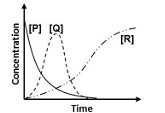
\includegraphics[width=0.45\columnwidth]{figs/q7a.png}
        \item 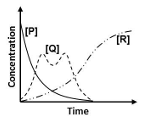
\includegraphics[width=0.45\columnwidth]{figs/q7b.png}
        \item 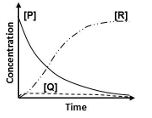
\includegraphics[width=0.45\columnwidth]{figs/q7c.png}
        \item 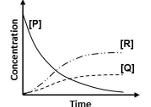
\includegraphics[width=0.45\columnwidth]{figs/q7d.png}
        \end{multicols}
        \hfill{\brak{\text{GATE CY-2013}}}
    \end{enumerate}



\item At 273 K and 10 bar, the Langmuir adsorption of a gas on a solid surface gave the fraction of surface coverage as 0.01. The Langmuir adsorption isotherm constant is \rule{1cm}{0.15mm} bar$^{-1}$. \brak{\text{Give the answer to the third decimal place}}
\hfill{\brak{\text{GATE CY-2013}}}



\item Conversion of boron trifluoride to tetrafluoroborate accompanies
    \begin{enumerate}
        \item increase in symmetry and bond elongation
        \item increase in symmetry and bond contraction
        \item decrease in symmetry and bond contraction
        \item decrease in symmetry and bond elongation
        \hfill{\brak{\text{GATE CY-2013}}}
    \end{enumerate}



\item The correct statement with respect to the bonding of the ligands, \ce{Me3N} and \ce{Me3P} with the metal ions \ce{Be^2+} and \ce{Pd^2+} is,
    \begin{enumerate}
        \item the ligands bind equally strong with both the metal ions as they are dicationic
        \item the ligands bind equally strong with both the metal ions as both the ligands are pyramidal
        \item the binding is stronger for \ce{Me3N} with \ce{Be^2+} and \ce{Me3P} with \ce{Pd^2+}
        \item the binding is stronger for \ce{Me3N} with \ce{Pd^2+} and \ce{Me3P} with \ce{Be^2+}
        \hfill{\brak{\text{GATE CY-2013}}}
    \end{enumerate}
\item A crystal has the lattice parameters a $\neq$ b $\neq$ c and $\alpha = \beta = \gamma = 90^{\circ}$. The crystal system is
\begin{enumerate}
    \item tetragonal
    \item monoclinic
    \item cubic
    \item orthorhombic
\end{enumerate}
\hfill \textbf{\brak{GATE CY-2013}}

\item The by-product formed in the characteristic reaction of \brak{CO}$_5$Cr=C\brak{OMe}\brak{Me} with MeNH$_2$ is
\begin{enumerate}
    \item CO
    \item MeOH
    \item MeCHO
    \item MeCONH$_2$
\end{enumerate}
\hfill \textbf{\brak{GATE CY-2013}}

\item The catalyst and co-catalyst used in the Wacker process, respectively, are
\begin{enumerate}
    \item PdCl$_2$ and Cu
    \item CuCl$_2$ and [PdCl$_4$]$^{2-}$
    \item Pd and CuCl
    \item [PdCl$_4$]$^{2-}$ and CuCl$_2$
\end{enumerate}
\hfill \textbf{\brak{GATE CY-2013}}

\item Oxymyoglobin Mb\brak{O_2} and oxyhemoglobin Hb\brak{O_2}$_4$, respectively, are
\begin{enumerate}
    \item paramagnetic and paramagnetic
    \item diamagnetic and diamagnetic
    \item paramagnetic and diamagnetic
    \item diamagnetic and paramagnetic
\end{enumerate}
\hfill \textbf{\brak{GATE CY-2013}}

\item Hapticity of cycloheptatriene in Mo\brak{C_7H_8}\brak{CO}$_3$ is \_\_\_\_\_\_.
\hfill \textbf{\brak{GATE CY-2013}}

\item The number of oxygen molecule\brak{s} that a molecule of hemerythrin can transport is \_\_\_\_\_\_.
\hfill \textbf{\brak{GATE CY-2013}}

\item The maximum number of stereoisomers possible for the compound given below is \_\_\_\_\_\_.
\begin{center}
    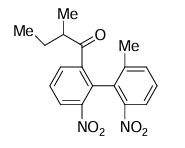
\includegraphics[width=0.3\columnwidth]{q17}
\end{center}
\hfill \textbf{\brak{GATE CY-2013}}

\item The correct sequence of the amino acids present in the tripeptide given below is
\begin{center}
    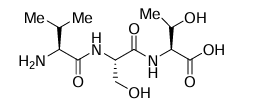
\includegraphics[width=0.5\columnwidth]{q18}
\end{center}
\begin{enumerate}
    \item Val-Ser-Thr
    \item Val-Thr-Ser
    \item Leu-Ser-Thr
    \item Leu-Thr-Ser
\end{enumerate}
\hfill \textbf{\brak{GATE CY-2013}}

\item Among the compounds given in the options A-D, the one that can be used as a formyl anion equivalent \brak{\text{in the presence of a strong base}} is
\begin{enumerate}
    \item ethylene
    \item nitroethane
    \item 1,3-dithiane
    \item 1,4-dithiane
\end{enumerate}
\hfill \textbf{\brak{GATE CY-2013}}

\item The major product formed in the reaction given below is
\begin{center}
    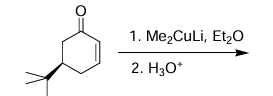
\includegraphics[width=0.5\columnwidth]{q20}
\end{center}
\begin{enumerate}
\begin{multicols}{4}
  \item 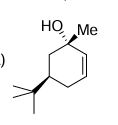
\includegraphics[width=0.5\columnwidth]{q20a}
    \item 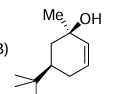
\includegraphics[width=0.5\columnwidth]{q20b}
    \item 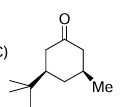
\includegraphics[width=0.5\columnwidth]{q20c}
    \item 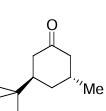
\includegraphics[width=0.5\columnwidth]{q20d}
    \end{multicols}
\end{enumerate}
\hfill \textbf{\brak{GATE CY-2013}}


\item The major product formed in the reaction given below is
    \begin{center} 
       
        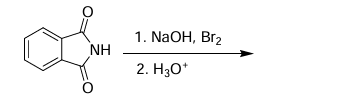
\includegraphics[width=0.6\columnwidth]{figs/q21.png}
    \end{center}
    \begin{enumerate}
        \begin{multicols}{2}
      
        \item 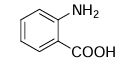
\includegraphics[width=0.4\columnwidth]{figs/q21a.png}
        \item 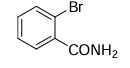
\includegraphics[width=0.4\columnwidth]{figs/q21b.png}
        \item 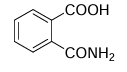
\includegraphics[width=0.4\columnwidth]{figs/q21c.png}
        \item 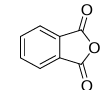
\includegraphics[width=0.4\columnwidth]{figs/q21d.png}
        \end{multicols}
        \hfill{\brak{\text{GATE CY-2013}}}
    \end{enumerate}



\item The pericyclic reaction given below is an example of
    \begin{center}
       
        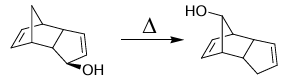
\includegraphics[width=0.4\columnwidth]{figs/q22.png}
    \end{center}
    \begin{enumerate}
        \begin{multicols}{2}
        \item [1,3]-sigmatropic shift
        \item [1,5]-sigmatropic shift
        \item [3,5]-sigmatropic shift
        \item [3,3]-sigmatropic shift
        \end{multicols}
        \hfill{\brak{\text{GATE CY-2013}}}
    \end{enumerate}



\item The major product formed in the reaction of quinoline with potassium amide \brak{\ce{KNH2}} in liquid ammonia is
    \begin{enumerate}
        \begin{multicols}{2}
       
        \item 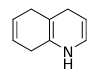
\includegraphics[width=0.3\columnwidth]{figs/q23a.png}
        \item 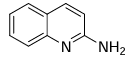
\includegraphics[width=0.3\columnwidth]{figs/q23b.png}
        \item 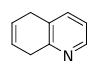
\includegraphics[width=0.3\columnwidth]{figs/q23c.png}
        \item 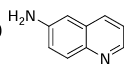
\includegraphics[width=0.3\columnwidth]{figs/q23d.png}
        \end{multicols}
        \hfill{\brak{\text{GATE CY-2013}}}
    \end{enumerate}



\item The number of signals that appear in the proton decoupled $^{13}$C NMR spectrum of benzonitrile \brak{\ce{C7H5N}} is \rule{1cm}{0.15mm}.
\hfill{\brak{\text{GATE CY-2013}}}



\item Among the compounds given in the options A-D, the one that exhibits a sharp band at around $3300\text{ cm}^{-1}$ in the IR spectrum is
    \begin{enumerate}
        \begin{multicols}{2}
        \item 1,2-butadiene
        \item 1,3-butadiene
        \item 1-butyne
        \item 2-butyne
        \end{multicols}
        \hfill{\brak{\text{GATE CY-2013}}}
    \end{enumerate}


\begin{center}
\section*{Q. 26 to Q. 55 carry two marks each.}

\end{center}

\item In the metathesis reaction given below, 4.32 g of the compound X was treated with 822 mg of the catalyst Y to yield 2.63 g of the product Z. The mol\% of the catalyst used in this reaction is \rule{1cm}{0.15mm}. [Atomic weights of Ru=101; P=31; Cl=35.51].
    \begin{center}
       
        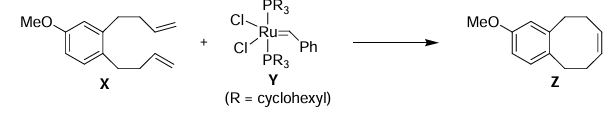
\includegraphics[width=0.8\columnwidth]{figs/q26.png}
    \end{center}
    \hfill{\brak{\text{GATE CY-2013}}}



\item An organic compound Q exhibited the following spectral data: \\
IR: $1760 \text{ cm}^{-1}$ \\
$^1$H NMR: $\delta$ \brak{ppm}: 7.2 \brak{1H, d, J=16.0 Hz}, 5.1 \brak{1 H, m}, 2.1 \brak{3 H, s}, 1.8 \brak{3H, d, J=7.0 Hz} \\
$^{13}$C NMR: $\delta$ \brak{ppm}: 170 \brak{\text{carbonyl carbon}}. \\
Compound Q is
    \begin{enumerate}
        \begin{multicols}{2}
        
        \item 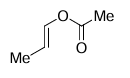
\includegraphics[width=0.35\columnwidth]{figs/q27a.png}
        \item 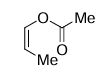
\includegraphics[width=0.35\columnwidth]{figs/q27b.png}
        \item 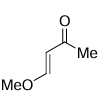
\includegraphics[width=0.35\columnwidth]{figs/q27c.png}
        \item 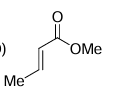
\includegraphics[width=0.35\columnwidth]{figs/q27d.png}
        \end{multicols}
        \hfill{\brak{\text{GATE CY-2013}}}
    \end{enumerate}



\item The major product formed in the Beckmann rearrangement of the compound given below is
    \begin{center}
     
        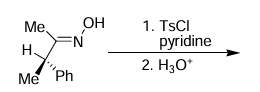
\includegraphics[width=0.6\columnwidth]{figs/q28.png}
    \end{center}
    \begin{enumerate}
        \begin{multicols}{2}
    
        \item 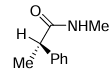
\includegraphics[width=0.4\columnwidth]{figs/q28a.png}
        \item 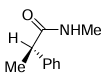
\includegraphics[width=0.4\columnwidth]{figs/q28b.png}
        \item 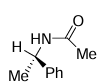
\includegraphics[width=0.4\columnwidth]{figs/q28c.png}
        \item 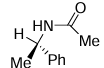
\includegraphics[width=0.4\columnwidth]{figs/q28d.png}
        \end{multicols}
        \hfill{\brak{\text{GATE CY-2013}}}
    \end{enumerate}



\item The major product formed in the reaction given below is
    \begin{center}
    
        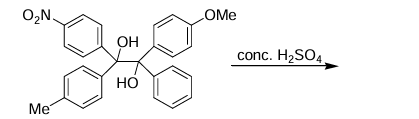
\includegraphics[width=0.5\columnwidth]{figs/q29.png}
    \end{center}
    \begin{enumerate}
        \begin{multicols}{2}
      
        \item 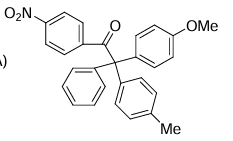
\includegraphics[width=0.35\columnwidth]{figs/q29a.png}
        \item 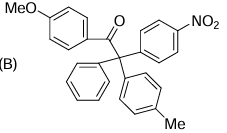
\includegraphics[width=0.35\columnwidth]{figs/q29b.png}
        \item 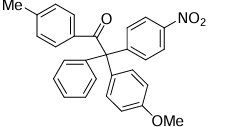
\includegraphics[width=0.35\columnwidth]{figs/q29c.png}
        \item 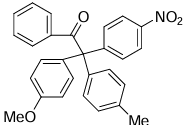
\includegraphics[width=0.35\columnwidth]{figs/q29d.png}
        \end{multicols}
        \hfill{\brak{\text{GATE CY-2013}}}
    \end{enumerate}



\item The major product formed in the reaction given below is
    \begin{center}
     
        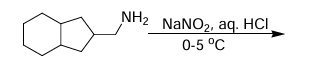
\includegraphics[width=0.5\columnwidth]{figs/q30.png}
    \end{center}
    \begin{enumerate}
        \begin{multicols}{2}
       
        \item 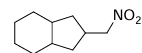
\includegraphics[width=0.3\columnwidth]{figs/q30a.png}
        \item 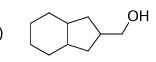
\includegraphics[width=0.3\columnwidth]{figs/q30b.png}
        \item 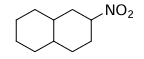
\includegraphics[width=0.3\columnwidth]{figs/q30c.png}
        \item 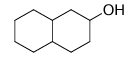
\includegraphics[width=0.3\columnwidth]{figs/q30d.png}
        \end{multicols}
        \hfill{\brak{\text{GATE CY-2013}}}
    \end{enumerate}

\item The major product\brak{s} formed in the reaction sequence given below is\brak{are}
    \begin{center}
      
        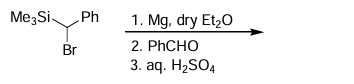
\includegraphics[width=0.7\columnwidth]{figs/q31.png}
    \end{center}
    \begin{enumerate}
      
        \item 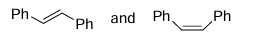
\includegraphics[width=0.4\columnwidth]{figs/q31a.png}
        \item 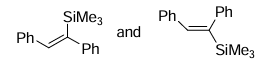
\includegraphics[width=0.4\columnwidth]{figs/q31b.png}
        \item 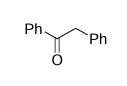
\includegraphics[width=0.25\columnwidth]{figs/q31c.png}
        \item 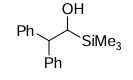
\includegraphics[width=0.25\columnwidth]{figs/q31d.png}
    
    \end{enumerate}
    \hfill{\brak{\text{GATE CY-2013}}}



\item Match the compounds in column I with the photochemical reactions that they can undergo given in column II.
    
    \begin{table}[H]
        \centering
        \begin{tabular}{m{5cm} m{8cm}}
            \textbf{Column I} & \textbf{Column II} \\
            \hline \\
            \brak{i} 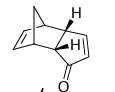
\includegraphics[width=1.5cm]{figs/q32a.png} & \brak{p} oxa-di-$\pi$-methane rearrangement \\ \\
            \brak{ii} 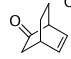
\includegraphics[width=2cm]{figs/q32b.png} & \brak{q} Paterno-Buchi reaction \\ \\
            \brak{iii} 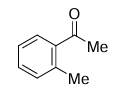
\includegraphics[width=2.5cm]{figs/q32c.png} & \brak{r} intramolecular [2+2]-cycloaddition \\ \\
             & \brak{s} photoenolisation \\
            \hline
        \end{tabular}
    \end{table}

    \begin{enumerate}
        \item \brak{i}-\brak{q}; \brak{ii}-\brak{s}; \brak{iii}-\brak{p}
        \item \brak{i}-\brak{r}; \brak{ii}-\brak{p}; \brak{iii}-\brak{s}
        \item \brak{i}-\brak{p}; \brak{ii}-\brak{r}; \brak{iii}-\brak{q}
        \item \brak{i}-\brak{r}; \brak{ii}-\brak{s}; \brak{iii}-\brak{p}
    \end{enumerate}
    \hfill{\brak{\text{GATE CY-2013}}}



\item $e^{-2x^{2}}$ is an eigen function of the operator $\brak{\frac{d^{2}}{dx^{2}}-16x^{2}}$. The corresponding eigen value is
    \begin{enumerate}
        \begin{multicols}{4}
        \item +4
        \item -4
        \item +2
        \item -2
        \end{multicols}
        \hfill{\brak{\text{GATE CY-2013}}}
    \end{enumerate}



\item The infrared spectrum of HCl gas shows an absorption band centered at $2885\text{ cm}^{-1}$. The zero point energy of HCl molecule under harmonic oscillator approximation is
    \begin{enumerate}
        \begin{multicols}{2}
        \item $2.8665\times10^{-22}\text{ J}$
        \item $2.8665\times10^{-20}\text{ J}$
        \item $5.7330\times10^{-22}\text{ J}$
        \item $5.7330\times10^{-20}\text{ J}$
        \end{multicols}
        \hfill{\brak{\text{GATE CY-2013}}}
    \end{enumerate}



\item For the reaction $\ce{X2O4\brak{l} -> 2XO2\brak{g}}$ at 298 K, given the values, $\Delta U=9\text{ kJ}$ and $\Delta S=84\text{ J K}^{-1}$, $\Delta G$ is
    \begin{enumerate}
        \begin{multicols}{2}
        \item -11.08 kJ
        \item +11.08 kJ
        \item -13.55 kJ
        \item +13.55 kJ
        \end{multicols}
        \hfill{\brak{\text{GATE CY-2013}}}
    \end{enumerate}



\item The change in enthalpy when 3 mol of liquid benzene transforms to the vapor state at its boiling temperature \brak{80^{\circ}\text{C}} and at 1 bar pressure is \rule{1cm}{0.15mm} kJ.
\hfill{\brak{\text{GATE CY-2013}}}



\item The moment of inertia of a homonuclear diatomic molecule is $7.5\times10^{-45}\text{ kg m}^{2}$. Its rotational partition function at 500 K is \rule{1cm}{0.15mm}.
\hfill{\brak{\text{GATE CY-2013}}}



\item For a reaction of the type $X\underset{k_{2}}{\stackrel{k_{1}}{\rightleftharpoons}}Y$, the correct rate expression is \brak{[X]_{0} and [X] correspond to the concentrations of X at time t=0 and t=t respectively}
    \begin{enumerate}
        \item $-\frac{d[X]}{dt}=k_{1}[X]_{0}-\brak{k_{1}+k_{2}}[X]$
        \item $-\frac{d[X]}{dt}=\brak{k_{1}+k_{2}}[X]-k_{2}[X]_{0}$
        \item $-\frac{d[X]}{dt}=\brak{k_{1}+k_{2}}[X]_{0}-k_{1}[X]$
        \item $-\frac{d[X]}{dt}=\brak{k_{1}-k_{2}}[X]-k_{1}[X]_{0}$
    \end{enumerate}
    \hfill{\brak{\text{GATE CY-2013}}}



\item The temperature dependence of partition functions are as follows:
    \begin{align*}
        q_{\text{translation}} &\propto T^{3/2} \\
        q_{\text{rotation}} &\propto T \text{ \brak{linear molecule}} \\
        q_{\text{rotation}} &\propto T^{3/2} \text{ \brak{non-linear molecule}} \\
        q_{\text{vibration}} &\propto T^{0}
    \end{align*}
    According to the conventional transition state theory \brak{CTST}, the temperature dependence of the Arrhenius pre-exponential factor for a reaction of the type given below is \\
    linear molecule + linear molecule $\rightarrow$ non-linear transition state $\rightarrow$ products
    \begin{enumerate}
        \begin{multicols}{4}
        \item $T^{-1}$
        \item $T^{0}$
        \item $T^{1}$
        \item $T^{2}$
        \end{multicols}
        \hfill{\brak{\text{GATE CY-2013}}}
    \end{enumerate}
    

    
\item Decarbonylation reaction of $[\text{cis-}\brak{\ce{CH3CO}}\text{Mn}\brak{^{13}\ce{CO}}\brak{\ce{CO}}_4]$ yields X, Y and Z, where $X=[\ce{\brak{CH3}Mn\brak{CO}5}]$; $Y=[\text{cis-}\brak{\ce{CH3}}\text{Mn}\brak{^{13}\ce{CO}}\brak{\ce{CO}}_4]$; $Z=[\text{trans-}\brak{\ce{CH3}}\text{Mn}\brak{^{13}\ce{CO}}\brak{\ce{CO}}_4]$. The molar ratio of the products \brak{X:Y:Z} in this reaction is
    \begin{enumerate}
        \begin{multicols}{4}
        \item 1:1:1
        \item 1:2:1
        \item 1:1:2
        \item 2:1:1
        \end{multicols}
        \hfill{\brak{\text{GATE CY-2013}}}
    \end{enumerate}

\item According to polyhedral electron count rule, the structure of $\ce{Rh6\brak{CO}16}$ is
    \begin{enumerate}
        \begin{multicols}{4}
        \item closo
        \item nido
        \item arachno
        \item hypho
        \end{multicols}
        \hfill{\brak{\text{GATE CY-2013}}}
    \end{enumerate}
    

    
\item The increasing order of melting points of the halides NaCl, CuCl and NaF is
    \begin{enumerate}
        \item CuCl < NaCl < NaF
        \item NaF < NaCl < CuCl
        \item NaF < CuCl < NaCl
        \item CuCl < NaF < NaCl
    \end{enumerate}
    \hfill{\brak{\text{GATE CY-2013}}}
    

    
\item The correct electronic configuration and spin only magnetic moment of $\ce{Gd^3+}$ \brak{\text{at. no. 64}} are
    \begin{enumerate}
        \item [Xe]$4f^7$ and 7.9 BM
        \item [Xe]$4f^7$ and 8.9 BM
        \item [Xe]$4f^6 5d^1$ and 7.9 BM
        \item [Rn]$5f^7$ and 7.9 BM
    \end{enumerate}
    \hfill{\brak{\text{GATE CY-2013}}}
    

    
\item Among the following octahedral complexes, the one that has the highest enthalpy of hydration is
    \begin{enumerate}
        \item $\ce{[Ca\brak{H2O}6]^2+}$
        \item $\ce{[Mn\brak{H2O}6]^2+}$
        \item $\ce{[V\brak{H2O}6]^2+}$
        \item $\ce{[Cr\brak{H2O}6]^2+}$
    \end{enumerate}
    \hfill{\brak{\text{GATE CY-2013}}}
    


\item A metal crystallizes in face-centered cubic lattice with a lattice parameter of 4.20 \AA. The shortest atom to atom contact distance in the lattice is
    \begin{enumerate}
        \begin{multicols}{2}
        \item 4.20 \AA
        \item 2.97 \AA
        \item 2.42 \AA
        \item 2.10 \AA
        \end{multicols}
        \hfill{\brak{\text{GATE CY-2013}}}
    \end{enumerate}
    


\item Polarographic method of analysis to obtain individual amounts of $\ce{Cu^2+}$ and $\ce{Cd^2+}$ in a given mixture of the two ions \brak{\ce{Cu^2+} and \ce{Cd^2+}} is achieved by measuring their
    \begin{enumerate}
        \item half-wave potentials
        \item migration currents
        \item decomposition potentials
        \item diffusion currents
    \end{enumerate}
    \hfill{\brak{\text{GATE CY-2013}}}
    


\item The ground state term of $\ce{[Ni\brak{H2O}6]^2+}$ is
    \begin{enumerate}
        \begin{multicols}{4}
        \item ${}^{3}T_{1g}$
        \item ${}^{3}T_{2g}$
        \item ${}^{3}A_{2g}$
        \item ${}^{4}T_{1g}$
        \end{multicols}
        \hfill{\brak{\text{GATE CY-2013}}}
    \end{enumerate}
\end{enumerate}

\subsection*{Common Data Questions}

\textbf{Common Data for Questions 48 and 49:}

N,N-Dimethylformamide \brak{DMF} gives different patterns of signals for the methyl protons when its $^1$H NMR spectrum is recorded at different temperatures.

\begin{enumerate}[resume]
\item Match the patterns of the NMR signals given in column I with temperatures given in the column II.
    
    \begin{table}[H]
        \centering
        \begin{tabular}{l l}
            \textbf{I} & \textbf{II} \\
            \hline
            \brak{i} Two singlets, for three protons each, at $\delta$ 2.87 and 2.97 ppm & \brak{x} $25^{\circ}\text{C}$ \\
            \brak{ii} One sharp singlet for six protons at $\delta$ 2.92 ppm & \brak{y} $120^{\circ}\text{C}$ \\
            \brak{iii} One broad signal for six protons & \brak{z} $150^{\circ}\text{C}$ \\
            \hline
        \end{tabular}
    \end{table}
    
    \begin{enumerate}
        \item \brak{i}-\brak{x}; \brak{ii}-\brak{y}; \brak{iii}-\brak{z}
        \item \brak{i}-\brak{x}; \brak{ii}-\brak{z}; \brak{iii}-\brak{y}
        \item \brak{i}-\brak{z}; \brak{ii}-\brak{x}; \brak{iii}-\brak{y}
        \item \brak{i}-\brak{z}; \brak{ii}-\brak{y}; \brak{iii}-\brak{x}
    \end{enumerate}
    \hfill{\brak{\text{GATE CY-2013}}}



\item Based on the above data, the calculated difference in the frequencies of the two methyl singlets, if the spectrum is recorded on a 300 MHz spectrometer, is \rule{1cm}{0.15mm} Hz.
\hfill{\brak{\text{GATE CY-2013}}}

\end{enumerate}



\textbf{Common Data for Questions 50 and 51:}

Heating a mixture of ammonium chloride and sodium tetrahydridoborate gives one liquid product\brak{X}, along with other products, under ambient conditions.

\begin{enumerate}[resume]
\item Compound X is
    \begin{enumerate}
        \item $\ce{NH4[BH4]}$
        \item $\ce{[\brak{NH3}2BH2][BH4]}$
        \item $\ce{N3B3H6}$
        \item $\ce{N3B3H12}$
    \end{enumerate}
    \hfill{\brak{\text{GATE CY-2013}}}

\item Compound X is an example of
    \begin{enumerate}
        \item ionic liquid
        \item saturated heterocycle
        \item molecular cage
        \item unsaturated heterocycle
    \end{enumerate}
    \hfill{\brak{\text{GATE CY-2013}}}
\end{enumerate}

\subsection*{Linked Answer Questions}

\textbf{Statement for Linked Answer Questions 52 and 53:}
\begin{enumerate}[resume]
\item The major product X formed in the reaction given below is
    \begin{center}
        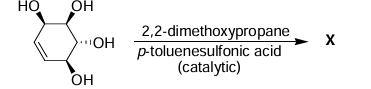
\includegraphics[width=0.8\columnwidth]{figs/q52.png}
    \end{center}
    \begin{enumerate}
      \begin{multicols}{2}
          
        \item \includegraphics[width=0.4\columnwidth]{figs/q52a.png}
        \item \includegraphics[width=0.4\columnwidth]{figs/q52b.png}
        \item \includegraphics[width=0.4\columnwidth]{figs/q52c.png}
        \item \includegraphics[width=0.4\columnwidth]{figs/q52d.png}
        \end{multicols}
    \end{enumerate}
    \hfill{\brak{\text{GATE CY-2013}}}



\item Oxidation of the product X, obtained in the above reaction, with active manganese dioxide, followed by acidic hydrolysis gives
    \begin{enumerate}
      \begin{multicols}{2}
        
        \item \includegraphics[width=0.4\columnwidth]{figs/q53a.png}
        \item \includegraphics[width=0.4\columnwidth]{figs/q53b.png}
        \item \includegraphics[width=0.4\columnwidth]{figs/q53c.png}
        \item \includegraphics[width=0.4\columnwidth]{figs/q53d.png}
        \end{multicols}
    \end{enumerate}
    \hfill{\brak{\text{GATE CY-2013}}}
\end{enumerate}



\textbf{Statement for Linked Answer Questions 54 and 55:}

The standard half-cell reduction potential of $\ce{Fe^3+\brak{aq} | Fe}$ is -0.036 V and that of $\ce{OH^{-}\brak{aq} | Fe\brak{OH}3\brak{s} | Fe}$ is -0.786 V.

\begin{enumerate}[resume]
\item For the determination of solubility product \brak{K_{\text{sp}}} of $\ce{Fe\brak{OH}3}$, the appropriate cell representation and its emf are, respectively,
    \begin{enumerate}
        \item $\ce{Fe | Fe\brak{OH}3\brak{s} | OH^{-}\brak{aq} || Fe^3+\brak{aq} | Fe}$, -0.750 V
        \item $\ce{Fe | Fe^3+\brak{aq} || OH^{-}\brak{aq} | Fe\brak{OH}3\brak{s} | Fe}$, -0.750 V
        \item $\ce{Fe | Fe\brak{OH}3\brak{s} | OH^{-}\brak{aq} || Fe^3+\brak{aq} | Fe}$, +0.750 V
        \item $\ce{Fe | Fe^3+\brak{aq} || OH^{-}\brak{aq} | Fe\brak{OH}3\brak{s} | Fe}$, -0.822 V
    \end{enumerate}
    \hfill{\brak{\text{GATE CY-2013}}}
    


\item The value of $\ln\brak{K_{\text{sp}}}$ for $\ce{Fe\brak{OH}3}$ at 298 K is
    \begin{enumerate}
        \begin{multicols}{4}
        \item -38.2
        \item +87.6
        \item -96.0
        \item -87.6
        \end{multicols}
    \end{enumerate}
    \hfill{\brak{\text{GATE CY-2013}}}
\end{enumerate}


\textbf{Q. 56 -- Q. 60 carry one mark each.}


\begin{enumerate}[resume]

\item If $3 \leq X \leq 5$ and $8 \leq Y \leq 11$ then which of the following options is TRUE?
    \begin{enumerate}
        \item $\frac{3}{5} \leq \frac{X}{Y} \leq \frac{8}{5}$
        \item $\frac{3}{11} \leq \frac{X}{Y} \leq \frac{5}{8}$
        \item $\frac{3}{11} \leq \frac{X}{Y} \leq \frac{8}{5}$
        \item $\frac{3}{5} \leq \frac{X}{Y} \leq \frac{8}{11}$
    \end{enumerate}
    \hfill{\brak{\text{GATE CY-2013}}}
    


\item The Headmaster \rule{2cm}{0.15mm} to speak to you. \\ Which of the following options is incorrect to complete the above sentence?
    \begin{enumerate}
        \item is wanting
        \item wants
        \item want
        \item was wanting
    \end{enumerate}
    \hfill{\brak{\text{GATE CY-2013}}}



\item Mahatama Gandhi was known for his humility as
    \begin{enumerate}
        \item he played an important role in humiliating exit of British from India.
        \item he worked for humanitarian causes.
        \item he displayed modesty in his interactions.
        \item he was a fine human being.
    \end{enumerate}
    \hfill{\brak{\text{GATE CY-2013}}}



\item All engineering students should learn \underline{mechanics}, \underline{mathematics} and \underline{how to do computation}. \\
\phantom{xxxxxxxxxxxxxxxxxxxxxxxxxxxxxxxxx}I \phantom{xxxxxxxxxxxx} II \phantom{xxxxxxxxxxxxxxxxxx} III \phantom{xxxxxxxxxx} IV \\
Which of the above underlined parts of the sentence is not appropriate?
    \begin{enumerate}
        \begin{multicols}{4}
        \item I
        \item II
        \item III
        \item IV
        \end{multicols}
    \end{enumerate}
    \hfill{\brak{\text{GATE CY-2013}}}



\item Select the pair that best expresses a relationship similar to that expressed in the pair: \\ water: pipe::
    \begin{enumerate}
        \item cart: road
        \item electricity: wire
        \item sea: beach
        \item music: instrument
    \end{enumerate}
    \hfill{\brak{\text{GATE CY-2013}}}

\textbf{Q.61 to Q.65 carry two  marks each}


\item Velocity of an object fired directly in upward direction is given by $v = 80 - 32t$, where $t$ \brak{time} is in seconds. When will the velocity be between 32 m/s and 64 m/s?
\begin{enumerate}
    \item \brak{1, 3/2}
    \item \brak{1/2, 1}
    \item \brak{1/2, 3/2}
    \item \brak{1, 3}
\end{enumerate}
\hfill \textbf{\brak{GATE CY-2013}}

\item In a factory, two machines M$_1$ and M$_2$ manufacture 60\% and 40\% of the auto-components respectively. Out of the total production, 2\% of M$_1$ and 3\% of M$_2$ are found to be defective. If a randomly drawn auto-component from the combined lot is found defective, what is the probability that it was manufactured by M$_2$?
\begin{enumerate}
    \item 0.35
    \item 0.45
    \item 0.5
    \item 0.4
\end{enumerate}
\hfill \textbf{\brak{GATE CY-2013}}

\item Following table gives data on tourists from different countries visiting India in the year 2011.

\begin{center}
\begin{tabular}{|c|c|}
\hline
Country & Number of Tourists \\
\hline
USA & 2000 \\
England & 3500 \\
Germany & 1200 \\
Italy & 1100 \\
Japan & 2400 \\
Australia & 2300 \\
France & 1000 \\
\hline
\end{tabular}
\end{center}

Which two countries contributed to one third of the total number of tourists who visited India in 2011?
\begin{enumerate}
    \item USA and Japan
    \item USA and Australia
    \item England and France
    \item Japan and Australia
\end{enumerate}
\hfill \textbf{\brak{GATE CY-2013}}

\item If $|-2x + 9| = 3$ then the possible value of $|-x| - x^2$ would be:
\begin{enumerate}
    \item 30
    \item -30
    \item -42
    \item 42
\end{enumerate}
\hfill \textbf{\brak{GATE CY-2013}}

\item All professors are researchers. Some scientists are professors. Which of the given conclusions is logically valid and inferred from the above arguments:
\begin{enumerate}
    \item All scientists are researchers
    \item All professors are scientists
    \item Some researchers are scientists
    \item No conclusion follows
\end{enumerate}
\hfill \textbf{\brak{GATE CY-2013}}

\end{enumerate}

\begin{center}
    
\textbf{END OF THE QUESTION PAPER}
\end{center} 




\end{document}


